% !TeX root = ../sustechthesis-example.tex

\chapter[量子计算]{量子计算\label{section:quantum_computation}}
% \textcolor{red}{
% 这部分从经典计算讲到量子计算,并简单介绍当前常见的实现量子计算的平台... 
% }
\section[量子计算基本原理介绍]{量子计算基本原理介绍}
% \textcolor{red}{主要参考文献\cite[]{Williams2011}}

目前,计算机的电路模型是计算过程最有用的抽象,广泛应用于计算机工业在实际计算硬件的设计和构建中。在电路模型中,计算机科学家将任何计算视为等同于由作用于某个二进制(\emph{比特串, Bit String})输入的少数不同类型的\emph{布尔逻辑门(Boolean Logic Gates)}构建的电路的动作。每个逻辑门根据门的定义以某种确定性的方式将其输入位转换为一个或多个输出位。通过组合计算电路图中的门,使前一级门的输出作为一级门的输入,计算机科学家可以证明这可以完成任何可行的计算\cite[]{Williams2011}。

\subsection[经典逻辑门]{经典逻辑门}
逻辑是数学的一个子领域,主要关注论点的有效性,即通过从起始假设(称为公理)进行推理过程来确定命题的真实性或虚假性,并通过对它们应用有效的推理规则。逻辑不关心确定现实世界中实际为真或假的内容,因为现实世界是但我们可能选择推理的无限多个可能世界之一。相反,逻辑提供了数学框架,我们可以从给定的开始假设中得出有效的结论。

经典计算机的数学基础是\emph{布尔代数(Boolean Algebra, BA)}\cite[]{Burris_2023}。\emph{BA}提供代数表达式的解释作为关于对象类的陈述。在\emph{BA}中,所有对象的全体是一个\emph{集合(Set)},而像$A$、$B$、$C$这样的\emph{符号(Symbols)}表示集合当中的\emph{子集合(Subset)}对象。然后集合上的一般操作,例如交集$A\cap B$、并集$A\cup B$和补集$A^c$可以表示为对这些子集对象的做出表述,如图\ref{fig:boolean_algebra}所示。
\begin{figure}
    \centering
    \caption[集合操作]{集合的并集、交集和补集运算的图形说明}
    \label{fig:boolean_algebra}
    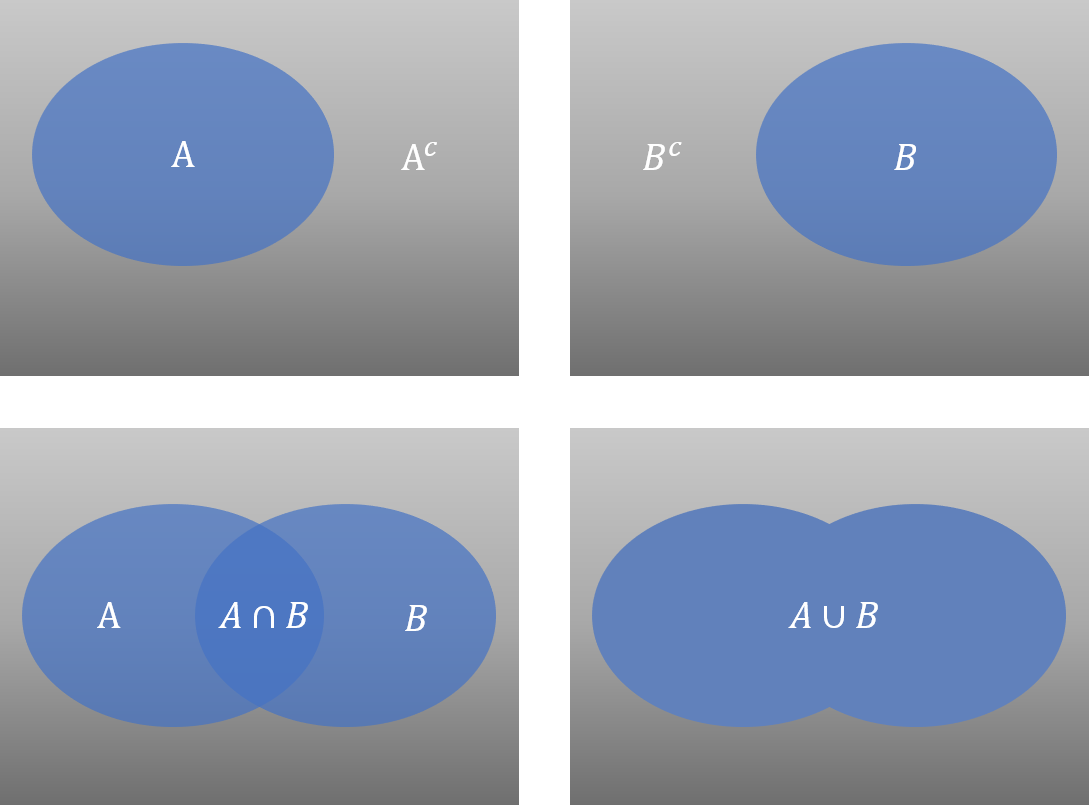
\includegraphics[width=1.0\linewidth]{boolean_algebra.png}
\end{figure}

举个简单的例子,如果$A$表示会打乒乓球的人,$B$表示会打篮球的人;则$A\cap B$表示既会打乒乓球又(AND)会打篮球的人;$A\cup B$表示所有会打乒乓球或者(OR)会打篮球的人;$A^c$表示所有所有不(NOT)会打乒乓球的人。

正如上面例中介绍到的,逻辑连接词$AND$、$OR$和$NOT$描述了由交集、并集和补集操作引起的集合的解释,表明\emph{集合操作(Set Operations)}和\emph{逻辑操作(Logic Operations)}之间存在密切的联系。

当我们能够将代数语句转化为逻辑语句后,我们就可以很容易地定义表示相同逻辑的不同代数。也就是用一个含有一系列用逻辑函数($AND,OR,NOT$)联系起来的变量($a,b,c,\dots$)的数学函数来表示一个或真或假的\emph{逻辑命题(Logical Proposition)}。
表\ref{tb:de_morgan_law}列出了部分所谓的\emph{De-Morgan定律(De-Morgan's Laws)},它给出了基本逻辑命题的句法等效版本。通过使用这些定律,我们可以从$\wedge$的所有实例或$\vee$的所有实例的任何逻辑表达式中系统地消除。这意味着我们可以将非常复杂的逻辑命题简化为形成两种标准形式之一,即连词的分离(即\emph{析取范式,Disjunctive Normal Form})或析取连词(即\emph{连词范式,Conjunctive Normal Form})。

因此,如果我们可以创建一些非常简单的基本门的硬件实现,例如,$NOT$, $AND$和$OR$,我们原则上可以将这些操作组合成非常复杂的电路。在经典的数字电路研究中包括许多这样的模块,比如加法器\cite[]{Mukherjee_Dhar_2014}、乘法器\cite[]{Shu_Haruo_2016}、滤波器\cite[]{Kumar_Agarwal_2021}等等,具体的相关内容将在后续章节进行介绍。

传统上,\emph{逻辑门(Logic Gate, LG)}被认为是一种接受一个或多个布尔值(即$FALSE$或$TRUE$)作为输入,并返回一个布尔值作为输出的物理设备。布尔值($FALSE$和$TRUE$)通常分别与位值$0$和$1$同义使用。逻辑门是现代计算机的关键部件。任何经典计算都可以分解成一系列逻辑门,每次只作用于几个比特。因此,逻辑门是所有现代计算机的核心。整体上各类基本的门电路可以分为两类:\emph{可逆门(Reversible Gate)}和\emph{不可逆门(Irreversible Gate)}。下面两小节将分别介绍他们。

\begin{table}
    \centering
    \caption[De-Morgan定律]{逻辑上等价的命题。这里通过使用\emph{De-Morgan定律},任何命题都可以单独使用$NOT$和$AND$表示,或者单独使用$NOT$和$OR$}
    \label{tb:de_morgan_law}
    \begin{tabular}[\linewidth]{L{8cm}L{4cm}}
        \toprule
        % % \rule{width}{height}
        % \rule{0pt}{1cm} %改变行高
        % \renewcommand\arraystretch{2}  % 2表示2倍行高,个人经验1.2比较好
        \textbf{逻辑等效形式} & \\
        \toprule 
        $a\wedge0=0$ & 0与\\
        $a\wedge1=a$ & 1与\\
        $a\vee 0=1$ & 0或\\
        $a\vee 1=a$ & 1或\\
        \midrule 
        $a\wedge a=a$ & 独立性\\
        $a\vee a=a$ & 独立性\\
        $a\wedge \neg a=0$ & 矛盾定理\\
        $a\vee \neg a=1$ & 无谓重复\\
        $ \neg \neg a=1$ & 双重否定\\
        \midrule 
        $a\vee b=b\vee a$ & 与的交换律\\
        $a\wedge b=b\wedge a$ & 或的交换律\\
        $a\vee (b\vee c)=(a\vee b)\vee c$ & 与的结合律\\
        $a\wedge (b\wedge c)=(a\wedge b)\wedge c$ & 或的结合律\\
        $a\wedge (b\vee c)=(a\wedge b)\vee (a\wedge c)$ & 分配律\\
        $a\vee (b\wedge c)=(a\vee b)\wedge (a\vee c)$ & 分配律\\
        \midrule
        $a\wedge (a\vee b)=a$ & 吸收律\\
        $a\vee (a\vee b)=a$ & 吸收律\\
        $a\wedge (\neg a\vee b)=a\vee b$ & 吸收律\\
        $a\vee (\neg a\vee b)=a\wedge b$ & 吸收律\\
        \midrule
        $\neg(a\wedge b)=(\neg a)\vee (\neg b)$ & De-Morgan定律\\
        $\neg(a\vee b)=(\neg a)\wedge (\neg b)$ & De-Morgan定律\\
        $(a\wedge b)\vee(a\wedge \neg b)=a$ & \\
        $a\Longrightarrow b=\neg a \vee b$ & \\
        $a\Longrightarrow b=\neg (a \vee \neg b)$ & \\
        \bottomrule
    \end{tabular}
\end{table}





\subsubsection[不可逆门:AND、OR、XOR]{不可逆门:AND、OR、XOR}

\begin{figure}
    \centering
    \caption[不可逻辑逆门]{不可逻辑逆门}
    \label{fig:irreversible_gates}
    \subcaptionbox{$AND$门图标\label{fig:and_gate}}{
        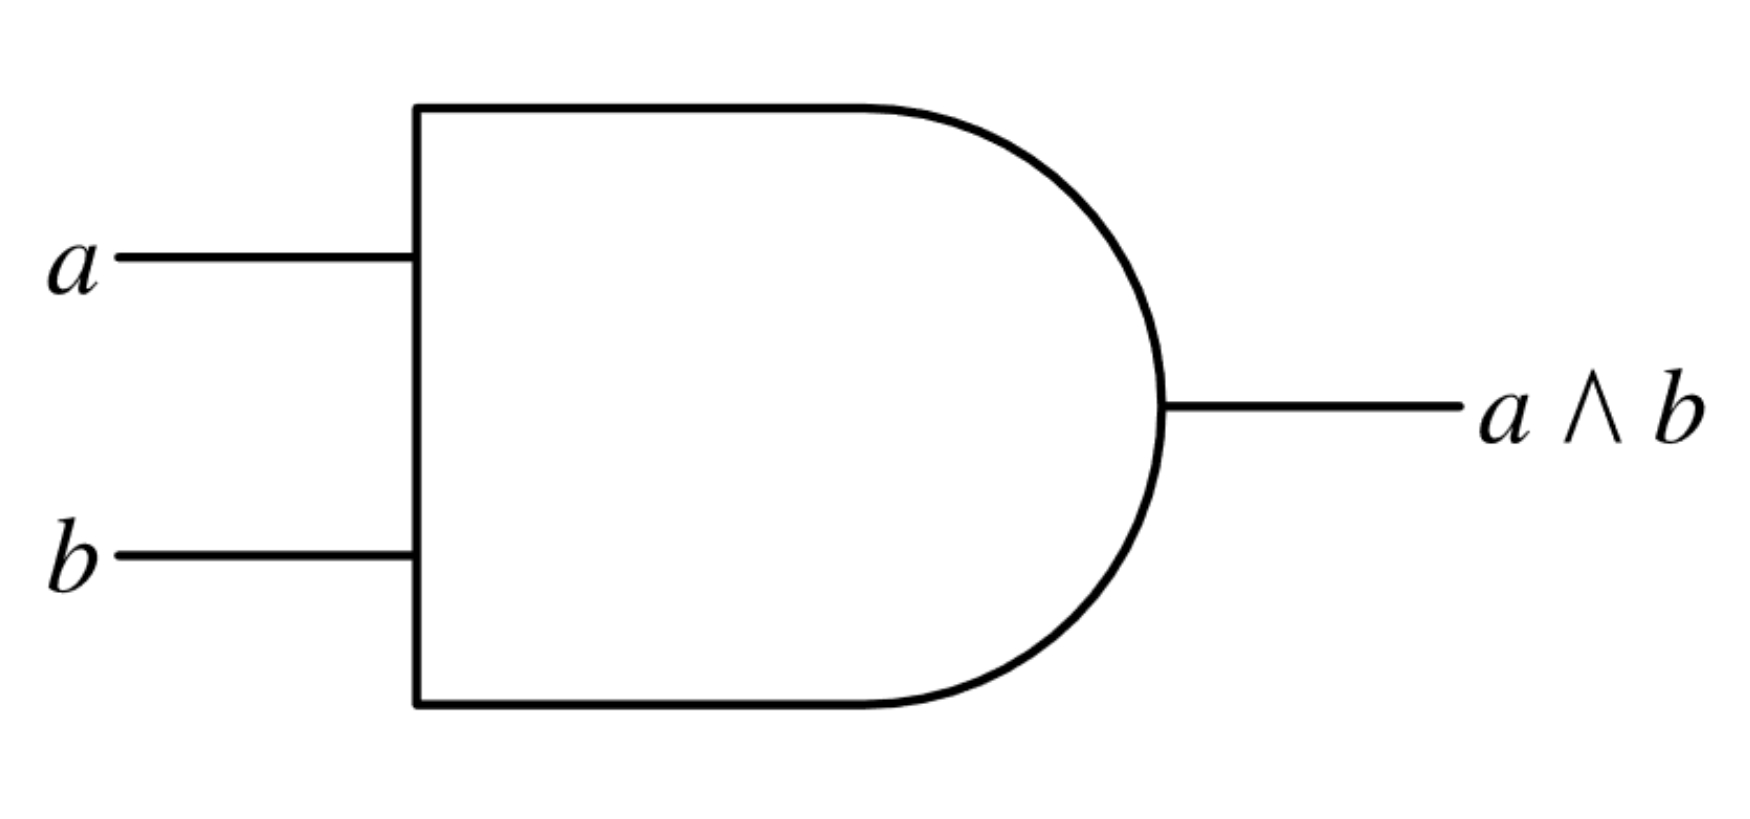
\includegraphics[width=0.3\linewidth]{and_gate.png}
    }
    \subcaptionbox{$OR$门图标\label{fig:or_gate}}{
        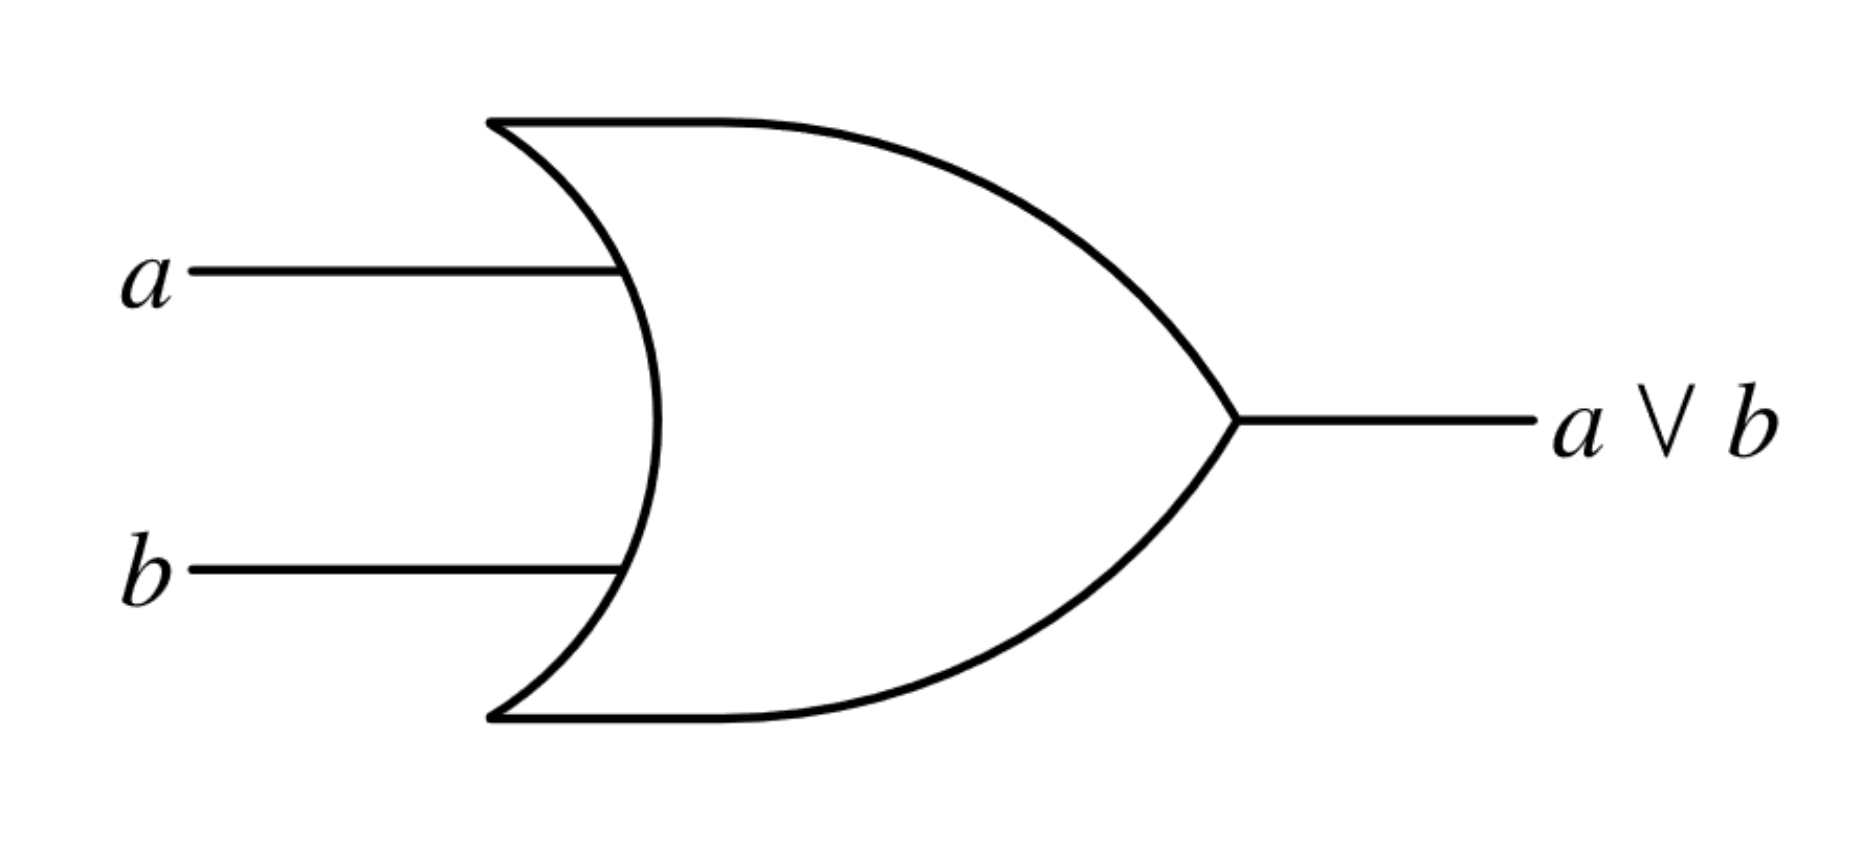
\includegraphics[width=0.3\linewidth]{or_gate.png}
    }
    \subcaptionbox{$XOR$门图标\label{fig:xor_gate}}{
        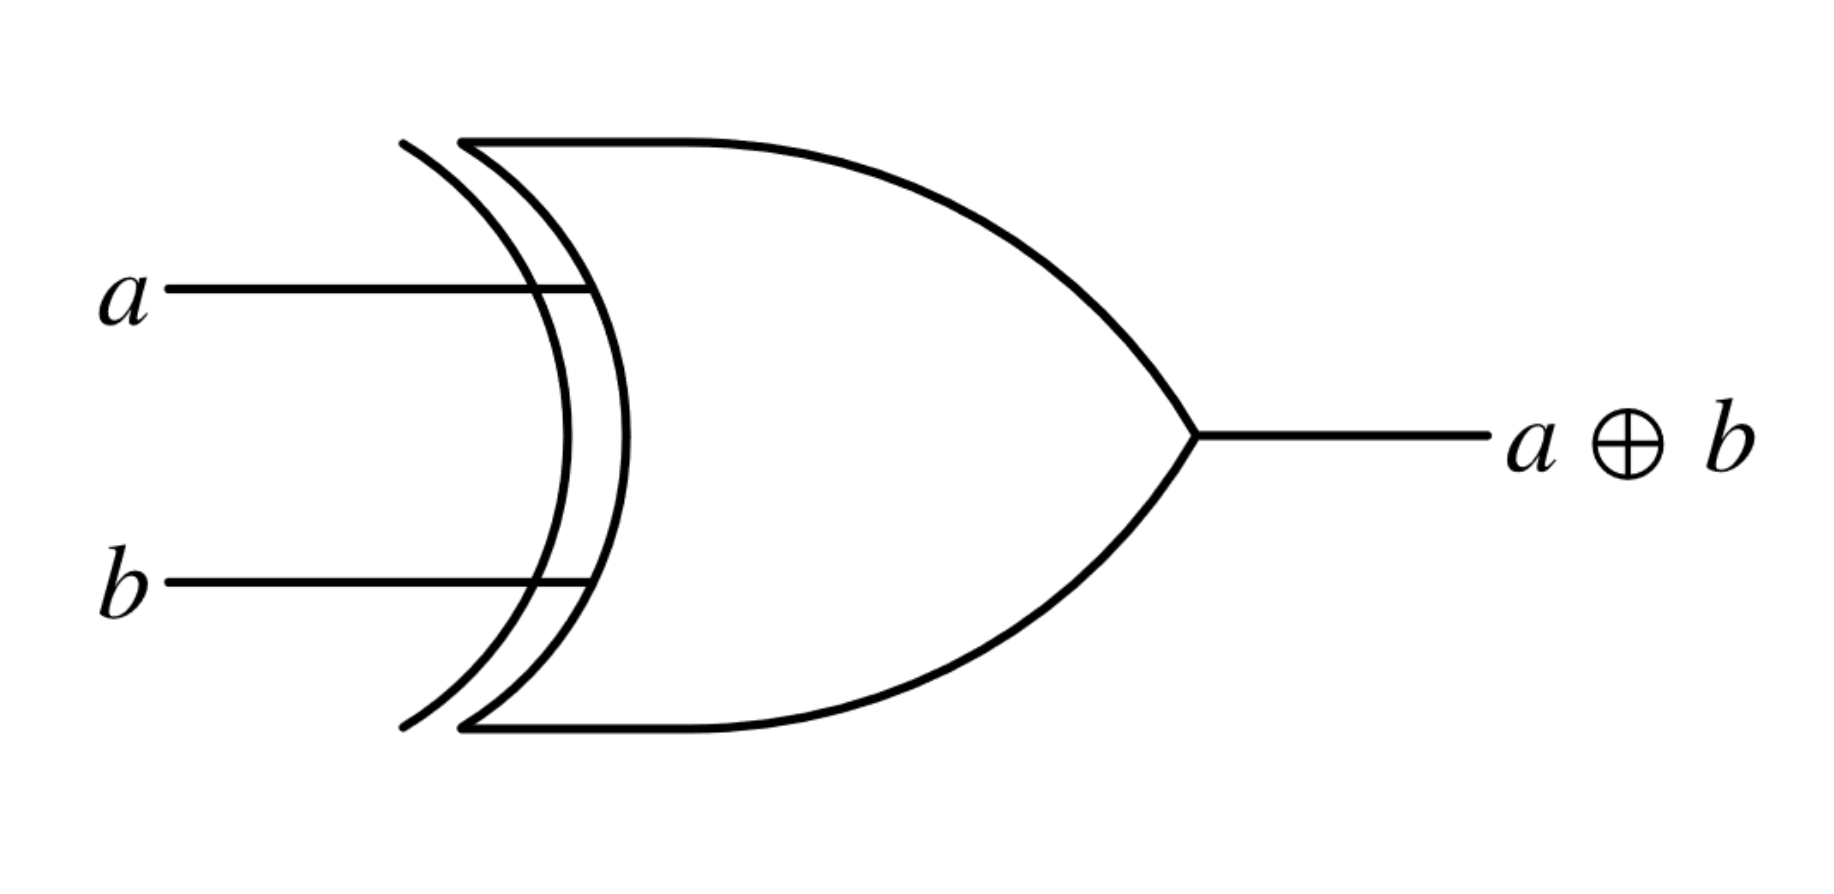
\includegraphics[width=0.3\linewidth]{xor_gate.png}
    }
\end{figure}

\begin{table}
    \centering
    \caption[不可逻辑逆门]{不可逻辑逆门}
    \subcaptionbox{$AND$门真值表\label{tb:and_gate}}{
        \begin{tabular}{C{1cm}C{1cm}C{1cm}}
            \toprule 
            \multicolumn{3}{c}{\textbf{AND}}\\
            \toprule
            a & b & $a\wedge b$ \\
            \hline
            0 & 0 & 0\\
            0 & 1 & 0\\
            1 & 0 & 0\\
            1 & 1 & 1\\
            \bottomrule
        \end{tabular}
    }
    \subcaptionbox{$OR$门的真值表\label{tb:or_gate}}{
        \begin{tabular}{C{1cm}C{1cm}C{1cm}}
            \toprule 
            \multicolumn{3}{c}{\textbf{OR}}\\
            \toprule
            a & b & $a\vee b$ \\
            \hline
            0 & 0 & 0\\
            0 & 1 & 1\\
            1 & 0 & 1\\
            1 & 1 & 1\\
            \bottomrule
        \end{tabular}
    }
    \subcaptionbox{$XOR$门的真值表\label{tb:xor_gate}}{
        \begin{tabular}{C{1cm}C{1cm}C{1cm}}
            \toprule 
            \multicolumn{3}{c}{\textbf{XOR}}\\
            \toprule
            a & b & $a\bigoplus b$ \\
            \hline
            0 & 0 & 0\\
            0 & 1 & 1\\
            1 & 0 & 1\\
            1 & 1 & 0\\
            \bottomrule
        \end{tabular}
    }
    
\end{table}


描述逻辑门动作的最好方法是用它的\emph{真值表(Truth Table)}。在真值表中,我们写下输入的所有可能的逻辑值及其相应的输出。例如,$AND$门的真值表如表\ref{tb:and_gate}所示。$AND$门在电路图中对应的图标如图\ref{fig:and_gate}所示。$AND$门在逻辑上是不可逆的,属于\emph{不可逆逻辑门(Irreversible Logic Gate, ILG)},这意味着我们无法为所有输出确定唯一的输入。具体来说,如果输出为$0$(即$FALSE$),则无法判断输入值是$00$、$01$还是$10$。换句话说,当$AND$门的输出为$0$时,它就会“擦除”一些信息。

同理,$OR$门的真值表如表\ref{tb:or_gate}所示。$OR$门对应的电路图标如图\ref{fig:or_gate}所示。$OR$门在逻辑上也是不可逆的,因为当它的输出为$1$(即$TRUE$)时,不可能说输入是$01$、$10$还是$11$。也就是说,当输出为$1$时,$OR$门再次擦除一些信息。

$OR$门有一种很常见变体,称为\emph{异或门(Exclusive-OR Gate)}(通常写为$XOR$或$\bigoplus$),事实证明它非常有用(因为很容易用晶体管实现)。$XOR$与$OR$相似,不同之处在于当两个输入都为$1$(即$TRUE$)时,它返回$0$(即$FALSE$)。$XOR$的真值表如表\ref{tb:xor_gate}所示。相应的异或电路图标如图\ref{fig:xor_gate}所示。




\subsubsection[可逆逻辑门:NOT、SWAP、CNOT]{可逆逻辑门:NOT、SWAP、CNOT\label{section:reversible_gates}}

上节介绍到的如$AND$门、$OR$门、$XOR$门等不可逆门在实践中应用十分广泛。随着数字芯片技术的不断发展,由于集成化的散热问题,不可逆门天然存在的限制逐渐被人们关注。基础物理理论告诉我们当信息被擦除时,一定伴随着能量的耗散\cite[]{Kastner_Schlatter_2023}。具体来说,每一比特信息的擦除会释放的能量为$kT\ln 2$,其中$k$是玻尔兹曼常数($k=1.3805\times 10^{-23}JK^{-1}$)而$T$是以\emph{凯尔文(Kelvin)}为单位的绝对温度。因此,即使所有其它能量损失机制从电路中消除了,由于信息擦除时发生的不可避免的能量损失,电路在操作时仍然会耗散能量。尽管当今在逻辑电路中由于逻辑不可逆性而导致的这种能量耗散与其它机制导致的能量耗散相比还比较小。然而,随着其它机制导致的能量耗散不断被克服,这种不可避免的信息擦除能量耗散将成为重要贡献,这将会阻碍计算芯片的进一步小型化和集成化。

克服上述问题的其中一个解决方案是修改现有的逻辑门使其仅使用\emph{可逆逻辑门(Reversible Logic Gate, RLG)}实现。在可逆逻辑门中,一个输入对应着一个确定的输出,反之亦然。因此,可逆门在起作用时永远不会删除任何信息,因此,可以向前运行基于可逆逻辑的计算以获得答案、复制的答案以及整个计算,然后再反向执行整个过程以恢复除用于复制中间点答案的小部分能量之外的所有能量。

可逆逻辑门的最简单例子是$NOT$门。$NOT$是一个\emph{1-input/1-output}门,它简单地反转它所处理的位值。$NOT$门的真值表如表\ref{tb:not_gate}所示。$NOT$门的电路图标如图\ref{fig:not_gate}所示。如果一个人知道输出位值,就可以明确地推断输入位值,反之亦然。

量子计算中非常重要的可逆门是\emph{受控非门($CNOT$)}。$CNOT$的真值表如表\ref{tb:cnot_gate}所示。$CNOT$门的电路图标如图2.9所示。$CNOT$门的效果是当且仅当第一个位设置为$1$时翻转第二个位的位值。也就是说,否定或不否定第二个位的决定由第一个位的值控制。这也是叫它受控非门的原因。
\begin{figure}
    \centering
    \caption[$NOT$门图标和真值表]{$NOT$门图标和真值表}
    \subcaptionbox{$NOT$门图标\label{fig:not_gate}}{
        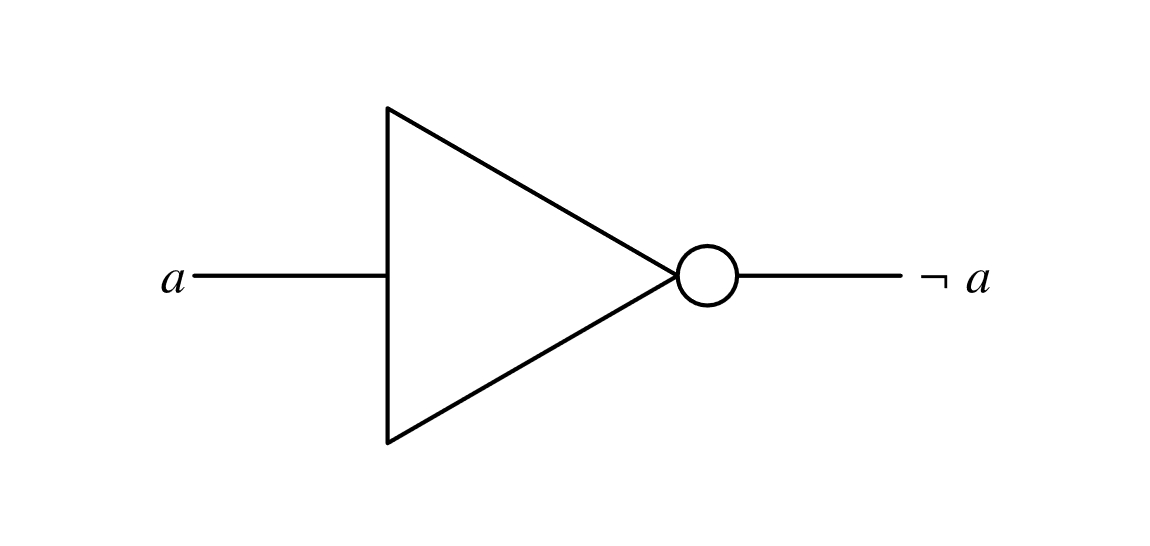
\includegraphics[width=0.45\linewidth]{not_gate.png}
    }
    \subcaptionbox{\emph{NOT}门真值表\label{tb:not_gate}}{
        \begin{tabular}{C{1.5cm}C{1.5cm}}
            \toprule 
            \multicolumn{2}{c}{\textbf{NOT}}\\
            \toprule
            a & $\neg a$  \\
            \hline
            0 & 1 \\
            1 & 0 \\
            \bottomrule
        \end{tabular}
    }
\end{figure}
% \begin{figure}
%     \centering
%     \caption{$NOT$门图标\label{fig:not_gate}}
%     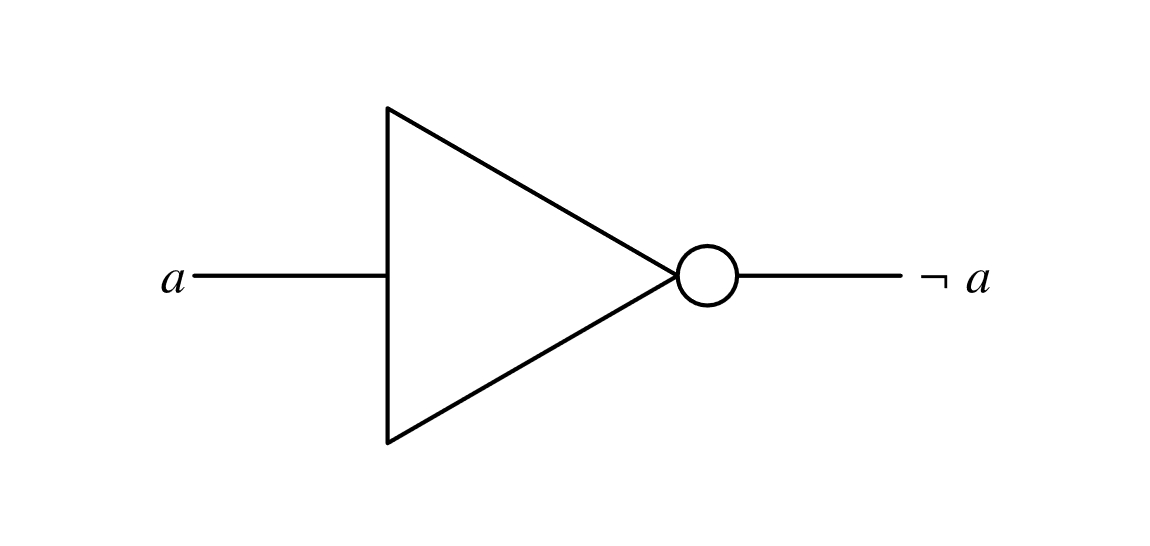
\includegraphics[width=0.8\linewidth]{not_gate.png}
% \end{figure}

% \begin{table}
%     \centering
%     \caption[\emph{NOT}门真值表]{\emph{NOT}门真值表\label{tb:not_gate}}
%     \begin{tabular}{C{1.5cm}C{1.5cm}}
%         \toprule 
%         \multicolumn{2}{c}{\textbf{NOT}}\\
%         \toprule
%         a & $\neg a$  \\
%         \hline
%         0 & 1 \\
%         1 & 0 \\
%         \bottomrule
%     \end{tabular}
% \end{table}

\begin{figure}
    \centering
    \caption[$CNOT$门图标和真值表]{$CNOT$门图标和真值表}
    \subcaptionbox{$CNOT$门图标\label{fig:cnot_gate}}{
        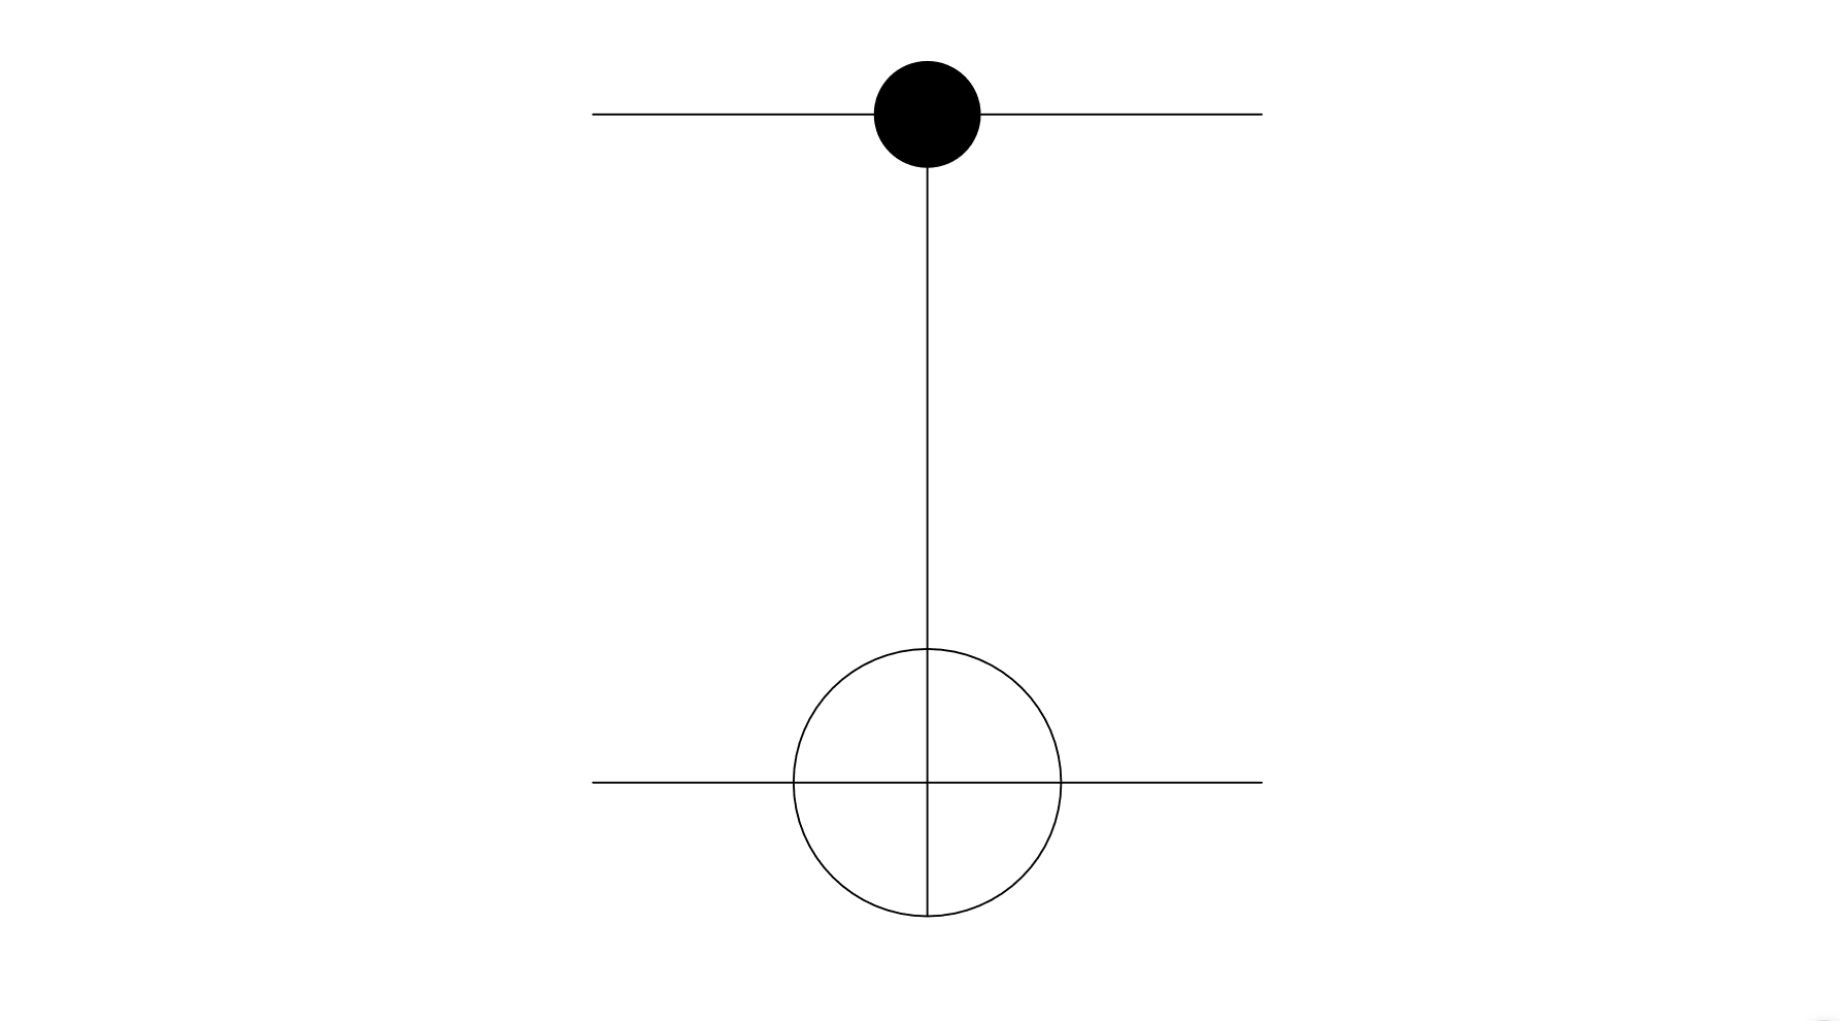
\includegraphics[width=0.45\linewidth]{cnot_gate}
    }
    \subcaptionbox{\emph{CNOT}门真值表\label{tb:cnot_gate}}{
        \begin{tabular}{C{1cm}C{1cm}C{1cm}C{1cm}}
            \toprule 
            \multicolumn{4}{c}{\textbf{CNOT}}\\
            \toprule
            a & b & $a'$ & $b'$  \\
            \hline
            0 & 0 & 0 & 0 \\
            0 & 1 & 1 & 0 \\
            1 & 0 & 0 & 1 \\
            1 & 1 & 1 & 1 \\
            \bottomrule
        \end{tabular}
    }
\end{figure}

% \begin{figure}
%     \centering
%     \caption{$CNOT$门图标\label{fig:cnot_gate}}
%     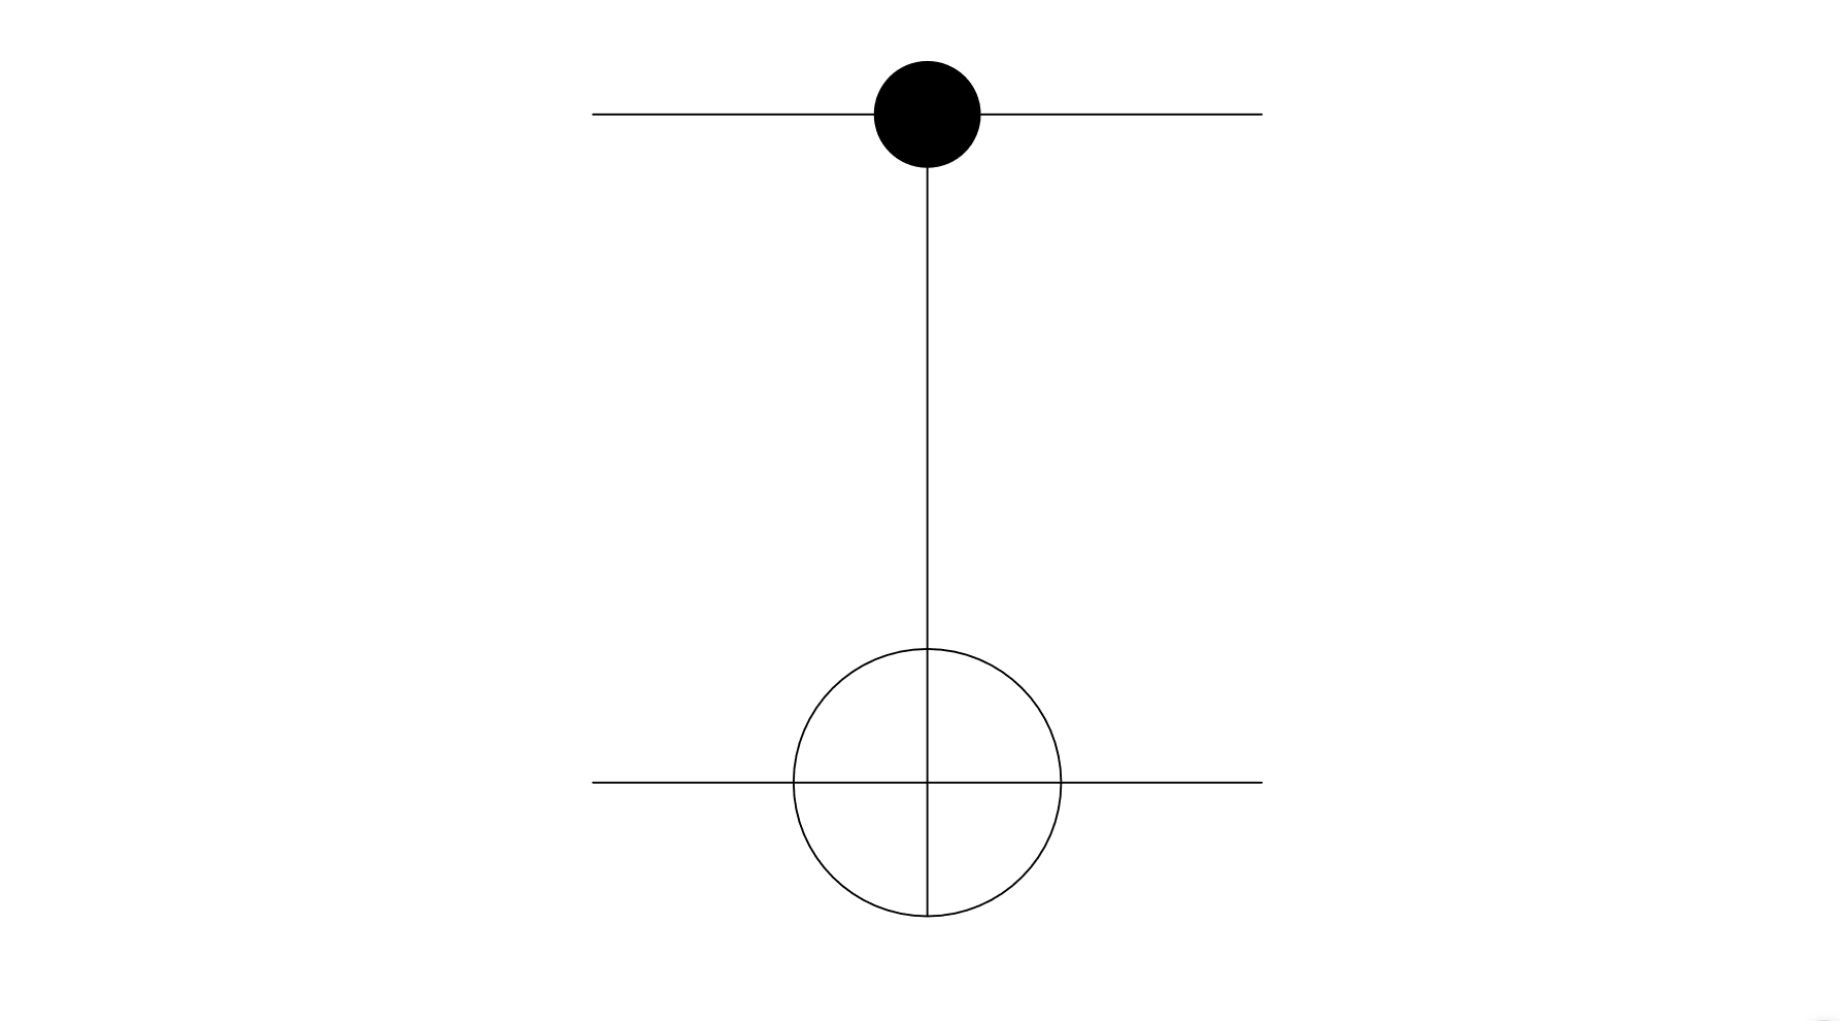
\includegraphics[width=0.8\linewidth]{cnot_gate.png}
% \end{figure}

% \begin{table}
%     \centering
%     \caption[\emph{CNOT}门真值表]{\emph{CNOT}门\label{tb:cnot_gate}}
%     \begin{tabular}{C{1cm}C{1cm}C{1cm}C{1cm}}
%         \toprule 
%         \multicolumn{4}{c}{\textbf{CNOT}}\\
%         \toprule
%         a & b & $a'$ & $b'$  \\
%         \hline
%         0 & 0 & 0 & 0 \\
%         0 & 1 & 1 & 0 \\
%         1 & 0 & 0 & 1 \\
%         1 & 1 & 1 & 1 \\
%         \bottomrule
%     \end{tabular}
% \end{table}

% \begin{figure}
%     \centering
%     \caption[可逆逻辑门]{可逆逻辑门}
%     \label{fig:reversible_gates}
%     \subcaptionbox{$NOT$门图标\label{fig:not_gate}}{
%         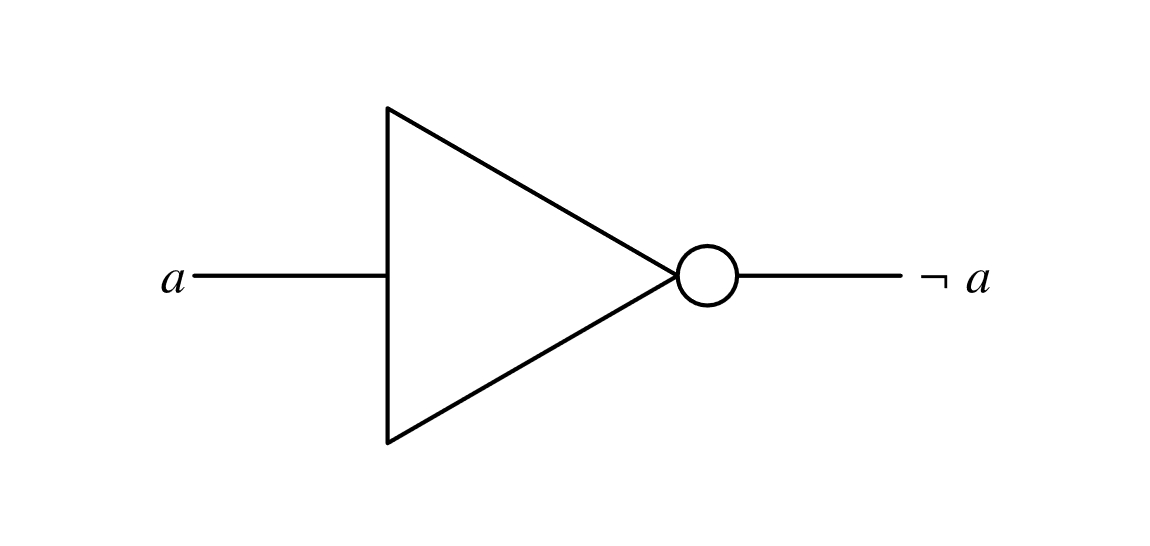
\includegraphics[width=0.45\linewidth]{not_gate.png}
%     }
%     \subcaptionbox{$CNOT$门图标\label{fig:cnot_gate}}{
%         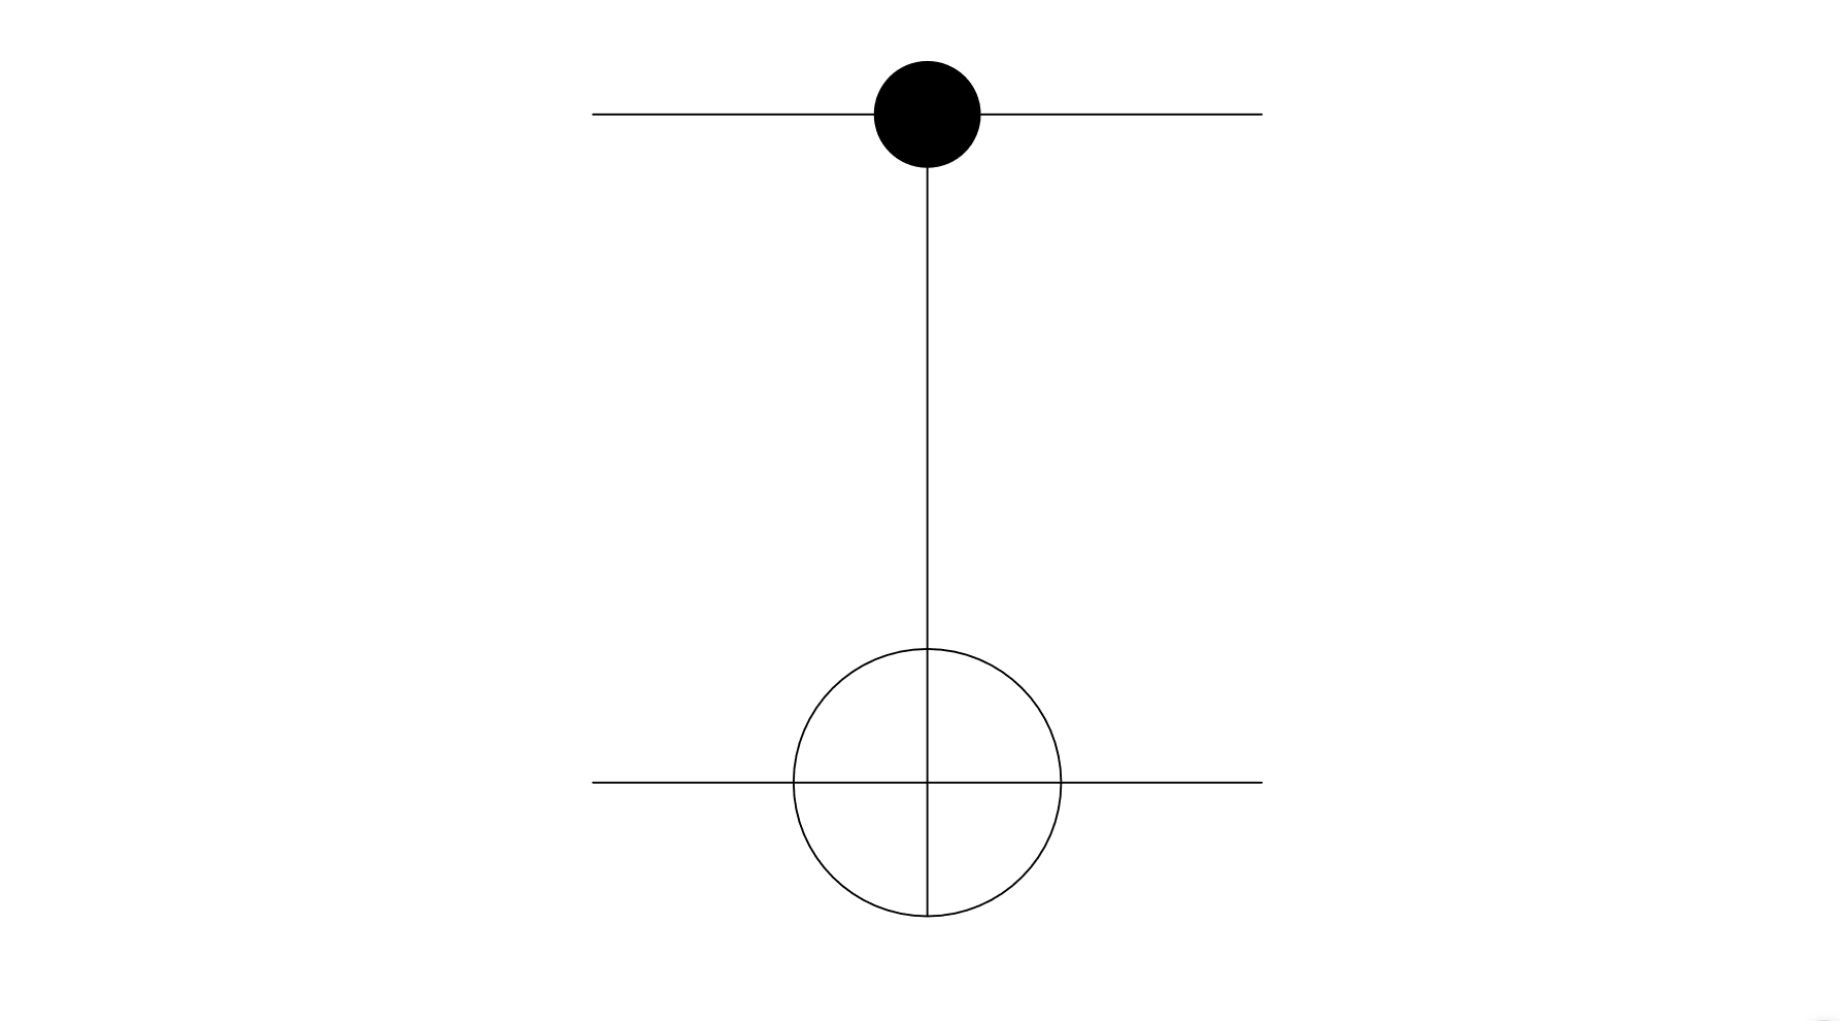
\includegraphics[width=0.45\linewidth]{cnot_gate.png}
%     }
% \end{figure}

% \begin{table}
%     \centering
%     \caption[可逆逻辑门]{可逆逻辑门}
%     \subcaptionbox{\emph{NOT}门\label{tb:not_gate}}{
%         \begin{tabular}{C{1.5cm}C{1.5cm}}
%             \toprule 
%             \multicolumn{2}{c}{\textbf{NOT}}\\
%             \toprule
%             a & $\neg a$  \\
%             \hline
%             0 & 1 \\
%             1 & 0 \\
%             \bottomrule
%         \end{tabular}
%     }
%     \subcaptionbox{\emph{CNOT}门\label{tb:cnot_gate}}{
%         \begin{tabular}{C{1cm}C{1cm}C{1cm}C{1cm}}
%             \toprule 
%             \multicolumn{4}{c}{\textbf{CNOT}}\\
%             \toprule
%             a & b & $a'$ & $b'$  \\
%             \hline
%             0 & 0 & 0 & 0 \\
%             0 & 1 & 1 & 0 \\
%             1 & 0 & 0 & 1 \\
%             1 & 1 & 1 & 1 \\
%             \bottomrule
%         \end{tabular}
%     }
% \end{table}




注意$CNOT$门不仅是一种RLG,还是一种\emph{通用逻辑门(Universal Logic Gate, ULG)}。也就是说以它为基础可以实现任何其它类型的门,比如$AND$、$OR$等等,进一步地可以只用$CNOT$搭建网络实现任何计算。ULG除了$CNOT$门外,还有$TOFFOLI$门\cite[]{Maslov_Dueck_Miller_2005}、$FREDKIN$门\cite[]{Adamatzky_2017}等等。$TOFFOLI$门和$FREDKIN$门都属于RLG,比如$TOFFOLI$门的真值表如表\ref{tb:toffoli_gate}所示,它的图标如图\ref{fig:toffoli_gate}所示。

\begin{figure}
    \centering
    \caption[TOFFOLI门图标和真值表]{TOFFOLI门图标和真值表}
    \subcaptionbox{\emph{TOFFOLI}门图标\label{fig:toffoli_gate}}{
        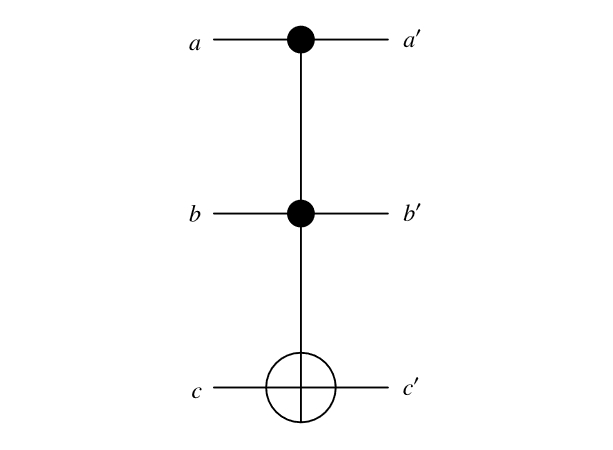
\includegraphics[width=0.45\linewidth]{toffoli_gate}
    }
    \subcaptionbox{\emph{TOFFOLI}门真值表\label{tb:toffoli_gate}}{
        \begin{tabular}{C{1cm}C{1cm}C{1cm}C{1cm}C{1cm}C{1cm}}
            \toprule
            a & b & c & $a'$ & $b'$ & $c'$\\
            \toprule 
            0 & 0 & 0 & 0 & 0 & 0\\
            0 & 0 & 1 & 0 & 0 & 1\\
            0 & 1 & 0 & 0 & 1 & 0\\
            0 & 1 & 1 & 0 & 1 & 1\\
            1 & 0 & 0 & 1 & 0 & 0\\
            1 & 0 & 1 & 1 & 0 & 1\\
            1 & 1 & 0 & 1 & 1 & 1\\
            1 & 1 & 1 & 1 & 1 & 0\\
            \bottomrule
        \end{tabular}
    }
\end{figure}

% \begin{table}
%     \centering
%     \caption[TOFFOLI门真值表]{\emph{TOFFOLI}门真值表}
%     \label{tb:toffoli_gate}
%     \begin{tabular}{C{1cm}C{1cm}C{1cm}C{1cm}C{1cm}C{1cm}}
%         \toprule
%         a & b & c & $a'$ & $b'$ & $c'$\\
%         \toprule 
%         0 & 0 & 0 & 0 & 0 & 0\\
%         0 & 0 & 1 & 0 & 0 & 1\\
%         0 & 1 & 0 & 0 & 1 & 0\\
%         0 & 1 & 1 & 0 & 1 & 1\\
%         1 & 0 & 0 & 1 & 0 & 0\\
%         1 & 0 & 1 & 1 & 0 & 1\\
%         1 & 1 & 0 & 1 & 1 & 1\\
%         1 & 1 & 1 & 1 & 1 & 0\\
%         \bottomrule
%     \end{tabular}
% \end{table}
% \begin{figure}
%     \centering
%     \caption[\emph{TOFFOLI}门图标]{\emph{TOFFOLI}门图标}
%     \label{fig:toffoli_gate}
%     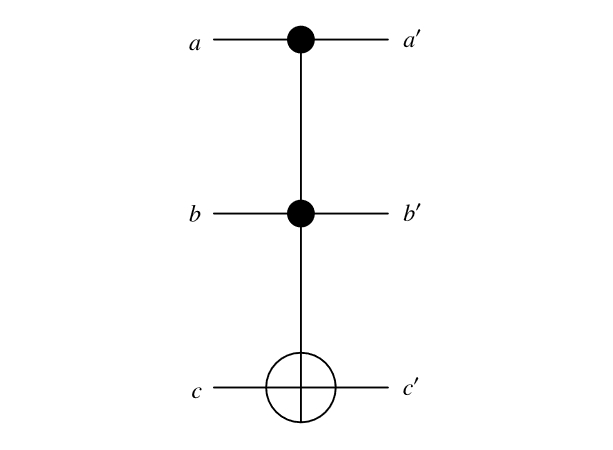
\includegraphics[width=0.8\linewidth]{toffoli_gate.png}
% \end{figure}

\subsection[量子逻辑门]{量子逻辑门}
前面我们已经讨论过经典的不可逆和经典的可逆门,这使我们能够更好地理解量子门的优越性。就像任何经典计算都可以分解成一系列经典逻辑门,这些门一次只作用于几个经典比特,因此任何量子计算也可以分解成一系列量子逻辑门,这些门一次只作用于几个量子比特。主要区别在于,虽然经典逻辑门操纵经典位值$0$或$1$,但量子门可以操纵任意多量子态,包括计算基态的任意叠加,这些量子态也经常纠缠在一起。因此,量子计算的逻辑门比经典计算的逻辑门更加多样化。

通常我们使用\emph{泡利矩阵(Pauli Matrices)},$\mathbb{1}, \mathbfit{X}, \mathbfit{Y}, \mathbfit{Z}$,来描述单量子比特。单量子比特既是厄米特(Hermitian)的也是幺正(Unitary)的,任何1-量子比特哈密顿量总是可以写成泡利矩阵的加权和:
\begin{align}
    \mathbb{1}=\begin{pmatrix}
        1 & 0 \\
        0 & 1 \\
    \end{pmatrix}, \quad \mathbfit{X}=\begin{pmatrix}
        0 & 1 \\
        1 & 0 \\
    \end{pmatrix}, \quad  \mathbfit{Y}=\begin{pmatrix}
        0 & -i \\
        i & 0 \\
    \end{pmatrix}, \quad  \mathbfit{Z}=\begin{pmatrix}
        1 & 0 \\
        0 & -1 \\
    \end{pmatrix} \label{eq:pauli_matrices}
\end{align}

实际上泡利矩阵$\mathbfit{X}$和经典逻辑门中的$NOT$门对应,有:
\begin{align}
    \mathbfit{X}\equiv NOT = \begin{pmatrix}
        0 & 1 \\
        1 & 0 \\
    \end{pmatrix}
\end{align}

也就是说$\mathbfit{X}$可以类似经典比特的$NOT$门用来翻转量子比特的状态,即:
\begin{align}
    \mathbfit{X}\ket{0}=\begin{pmatrix}
        0 & 1 \\
        1 & 0 \\
    \end{pmatrix}\cdot \begin{pmatrix}
         1 \\
         0 \\
    \end{pmatrix}=\begin{pmatrix}
        0 \\
        1 \\
   \end{pmatrix}=\ket{1}\\
   \mathbfit{X}\ket{1}=\begin{pmatrix}
    0 & 1 \\
    1 & 0 \\
\end{pmatrix}\cdot \begin{pmatrix}
     0 \\
     1 \\
\end{pmatrix}=\begin{pmatrix}
    1 \\
    0 \\
\end{pmatrix}=\ket{0}\\
\end{align}

但是注意$\mathbfit{X}$并不是一个真正意义上的\emph{量子非门(Quantum Not Gate, QNG)},实际上并不存在一个通用的QNG。

有一个很重要的量子门值得在这里被介绍,它就是\emph{Hadamard门(Hadamard Gate)},它的定义如下\cite[]{PRUDÊNCIO_2013}:
\begin{align}
    \mathbfit{H}=\frac{1}{\sqrt{2}}\begin{pmatrix}
        1 & 1 \\
        1 & -1 \\
    \end{pmatrix}
\end{align}

它的最广泛的应用是用来制备量子叠加态,基本的过程示意如下:
\begin{align}
    \mathbfit{H}\ket{0}=\frac{1}{\sqrt{2}}\begin{pmatrix}
        \ket{0}+\ket{1}
    \end{pmatrix}\\
    \mathbfit{H}\ket{1}=\frac{1}{\sqrt{2}}\begin{pmatrix}
        \ket{0}-\ket{1}
    \end{pmatrix}\\
\end{align}

这是一个看似简单的看门,但它有一个重要的性质。进一步地,它可以制备$n$个比特的叠加态,这些态将会均匀地分布在$[0, 1, ..., 2^n-1]$的范围上:
\begin{align}
    \mathbfit{H}\ket{0}\otimes\mathbfit{H}\ket{0}\otimes\dots\otimes\mathbfit{H}\ket{0}=\frac{1}{\sqrt{2^n}}\sum_{j=0}^{2^n-1}\ket{j}
\end{align}

其中$\ket{j}$是是由二进制数索引的计算基态,该二进制数将对应于 十进制符号中的数字$j$。比如对于$3$量子比特的寄存器来说,$\ket{0}$表示计算基态$\ket{000}$;$\ket{1}$表示计算基态$\ket{001}$;··· ;$\ket{7}$表示计算基态$\ket{111}$。

这些本征态意味着可以使用$n$比特同时写入的所有可能比特串组合。它实际上是量子计算最重要的技巧之一,因为它实现了仅使用多项式多次操作而将指数多的索引加载到量子计算机中。如果自然界没有种方法,我们则必须像我们在经典计算中所做的那样一个一个单独输入不同的位串,那么量子计算在计算复杂性方面取得突破的可能性要小得多。

在量子门的阐述中有一个门是绝对不能忽略的,那就是量子$CNOT$门。和经典$CNOT$门一样,它会根据一个比特的状态来决定是否翻转两一个比特的状态,比如:
\begin{align}
    \ket{00}\overset{CNOT}{\longrightarrow}\ket{00}\\
    \ket{01}\overset{CNOT}{\longrightarrow}\ket{01}\\
    \ket{10}\overset{CNOT}{\longrightarrow}\ket{11}\\
    \ket{11}\overset{CNOT}{\longrightarrow}\ket{10}\\
\end{align}

其中第二个比特(靠右的)的状态受到第一个比特(靠左的)的状态控制。由于$CNOT$门是一个通用的门,因此只要一个量子物理体系能够实现$CNOT$门,那么这个体系就具备了实现通用量子计算机的前景\cite[]{Zajac_Sigillito_Russ_Borjans_Taylor_Burkard_Petta_2018,Zhu_Cheng_Zhu_Chen_Guan_2022}。


\subsection[量子算法]{量子算法}









\section[量子计算的不同实现平台]{量子计算的不同实现平台}
\textcolor{red}{这部分需要分别找各个平台的文献进行整理,每个平台找一到两篇吧}
\subsection[离子量子计算]{离子量子计算}

\subsection[超导量子计算]{超导量子计算}

\subsection[原子量子计算]{原子量子计算}

\subsection[硅基量子计算]{硅基量子计算}

\subsection[光量子计算]{光量子计算}

\subsection[拓扑量子计算]{拓扑量子计算}






